\documentclass[aspectratio=169, table]{beamer}

\usepackage{array}
\usepackage{colortbl}
\usepackage{tabularx}
\usepackage{xcolor}
\usepackage{tikz}
\usetikzlibrary{arrows.meta, positioning, calc, fit}

\makeatletter
\def\input@path{{../theme/}}
\makeatother
\graphicspath{{../theme/}{../../figures/}}
\usetheme{Pradita}

\newcommand{\sectionframe}[1]{%
  \begin{frame}{\hfill}
    \centering
    \Huge{\textbf{#1}}
  \end{frame}
}

\newcommand{\takeaway}[1]{%
  \vspace{4pt}
  {\footnotesize #1}
}

\title{\LARGE Lapisan Implementasi \& Migrasi\\
  \vspace{8pt}
  pada ArchiMate}
\subtitle{IT30713 - Enterprise \& Platform Architecture}
\author{\textbf{Alfa Yohannis}}
\date{25 Juli 2026}

\begin{document}

\frame{\titlepage}

\begin{frame}[fragile]
  \frametitle{Contents}
  \vspace{20pt}
  \begin{columns}[t]
    \column{0.5\textwidth}
    \tableofcontents[sections={1-4}]

    \column{0.5\textwidth}
    \tableofcontents[sections={5-8}]
  \end{columns}
\end{frame}

\begin{frame}{\hfill}
  \centering
  \Huge{\textbf{Jika desain arsitektur target sudah lengkap, bagaimana mencapainya?}}
\end{frame}

% ============================================================
\section{Orientasi Bab}
\sectionframe{Orientasi Bab}

\begin{frame}{Tujuan Pembelajaran}
  \vspace{6pt}
  \begin{itemize}
    \item Menjelaskan elemen \textbf{lapisan implementasi \& migrasi} ArchiMate:
          \emph{work package}, \emph{deliverable}, \emph{event}, \emph{plateau},
          \emph{gap}.
    \item Menyusun \textbf{peta jalan} (\emph{roadmap}): rangkaian plateau dari
          \emph{baseline} ke \emph{target}.
    \item Menempatkan analisis dalam \textbf{TOGAF ADM Fase E (Peluang \& Solusi)}
          dan \textbf{Fase F (Perencanaan Migrasi)}.
    \item Menutup rantai keterlacakan \textbf{seluruh buku}: dari motivasi sampai
          paket kerja yang membangunnya.
  \end{itemize}
  \takeaway{Arah sesi: dari ``arsitektur target apa'' menuju ``bagaimana mencapai
  target itu, bertahap''.}
\end{frame}

\begin{frame}{Ringkasan Awal Bab}
  \vspace{6pt}
  \begin{itemize}
    \item Lapisan ini menjawab \textbf{bagaimana mencapai} target: langkah demi
          langkah, tanpa mengganti semuanya sekaligus.
    \item Pola inti: \textbf{work package mewujudkan deliverable}; \textbf{deliverable
          mewujudkan plateau}; \textbf{gap} = selisih baseline--target.
    \item Studi kasus: peta jalan rel Transfer---Baseline $\rightarrow$ MVP
          $\rightarrow$ Target (SNAP BI penuh).
    \item Keluaran memperkuat \textbf{Rekomendasi \& Rencana} makalah; menutup
          keseluruhan model.
  \end{itemize}
  \takeaway{Ini lapisan terakhir: menutup rantai motivasi $\rightarrow$ strategi
  $\rightarrow$ \dots $\rightarrow$ teknologi $\rightarrow$ implementasi.}
\end{frame}

% ============================================================
\section{Mengapa Lapisan Implementasi}
\sectionframe{Mengapa Lapisan Implementasi \& Migrasi}

\begin{frame}{Lapisan Implementasi \& Migrasi}
  \vspace{2pt}
  \centering
  \scalebox{0.74}{
    \begin{tikzpicture}[
      font=\small\bfseries,
      node distance=2.2mm,
      layer/.style={draw, rounded corners=1.5mm, align=left, minimum width=82mm,
        minimum height=10mm, inner xsep=4mm},
      strat/.style={layer, fill=orange!16},
      biz/.style={layer, fill=praditagreen!22},
      app/.style={layer, fill=blue!16},
      tech/.style={layer, fill=praditagreen!16},
      impl/.style={layer, fill=red!22, draw=red!55!black, line width=0.6mm},
    ]
      \node[strat] (s) {STRATEGI\\
        \footnotesize\mdseries Sumber daya, kapabilitas, arah tindakan};
      \node[biz, below=of s] (b) {BISNIS\\
        \footnotesize\mdseries Aktor, peran, proses, layanan, objek bisnis};
      \node[app, below=of b] (a) {APLIKASI\\
        \footnotesize\mdseries Komponen, layanan, fungsi, antarmuka, objek data};
      \node[tech, below=of a] (t) {TEKNOLOGI (\& FISIK)\\
        \footnotesize\mdseries Node, device, system software, artefak, jaringan};
      \node[impl, below=of t] (i) {IMPLEMENTASI \& MIGRASI \quad$\leftarrow$ \emph{fokus sesi ini}\\
        \footnotesize\mdseries \textbf{Work package, deliverable, event, plateau, gap}};
      \node[draw, rounded corners=2mm, fill=purple!22, align=center,
        text width=16mm, minimum height=60mm, right=5mm of a, font=\bfseries]
        (mot) {M\\O\\T\\I\\V\\A\\S\\I\\[2mm]\footnotesize\mdseries (mengapa)};
    \end{tikzpicture}
  }

  \takeaway{Lapisan ini melintasi semua lapisan: menyusun \emph{kapan} dan
  \emph{dengan apa} arsitektur target dibangun. Dipetakan ke fase \textbf{E \& F}.}
\end{frame}

\begin{frame}{Pola Migrasi (Plateau \& Gap)}
  \vspace{2pt}
  \centering
  \scalebox{1.0}{
    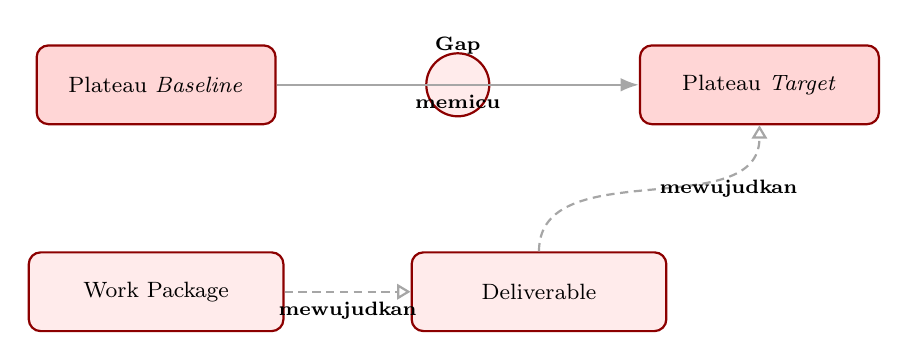
\begin{tikzpicture}[
      font=\footnotesize,
      impl/.style={rectangle, rounded corners=1.5mm, draw=red!55!black, fill=red!8,
        thick, align=center, text width=30mm, minimum height=10mm},
      plat/.style={rectangle, rounded corners=1.5mm, draw=red!55!black, fill=red!16,
        thick, align=center, text width=28mm, minimum height=10mm},
      real/.style={-{Triangle[open]}, thick, draw=gray!70, densely dashed},
      trig/.style={-Latex, thick, draw=gray!70},
      assoc/.style={thick, draw=gray!60}
    ]
      \node[plat] (p0) {Plateau \emph{Baseline}};
      \node[plat, right=46mm of p0] (p2) {Plateau \emph{Target}};
      \node[impl, below=16mm of p0] (wp) {Work Package};
      \node[impl, right=16mm of wp] (del) {Deliverable};
      \node[draw=red!55!black, fill=red!8, thick, circle, minimum size=8mm,
        inner sep=0pt] (gap) at ($(p0)!0.5!(p2)$) {};
      \node[font=\scriptsize\bfseries] at ($(gap)+(0,5mm)$) {Gap};
      \draw[trig] (p0) -- node[below,font=\scriptsize\bfseries]{memicu} (p2);
      \draw[real] (wp) -- node[below,font=\scriptsize\bfseries]{mewujudkan} (del);
      \draw[real] (del.north) to[out=90,in=-90] node[right,font=\scriptsize\bfseries]{mewujudkan} (p2.south);
    \end{tikzpicture}
  }

  \takeaway{Gap = \emph{apa} yang kurang; work package = \emph{siapa mengerjakan
  apa}; deliverable mewujudkan \textbf{plateau}---keadaan bernilai yang dicapai.}
\end{frame}

% ============================================================
\section{TOGAF ADM Fase E \& F}
\sectionframe{TOGAF ADM Fase E \& F:\\ Peluang, Solusi, dan Migrasi}

\begin{frame}{Siklus TOGAF ADM}
  \vspace{8pt}
  \begin{columns}[c]
    \column{0.4\textwidth}
    \centering
    \scalebox{0.85}{
      \begin{tikzpicture}[
        font=\footnotesize\bfseries,
        phase/.style={circle, draw=praditagreen, line width=0.4mm,
          fill=praditagreen!15, minimum size=11mm, inner sep=0pt},
        reqman/.style={circle, draw=blueColor, line width=0.4mm, fill=blueColor!15,
          minimum size=21mm, inner sep=1pt, align=center, font=\scriptsize\bfseries},
        prelim/.style={circle, draw=orange!80!black, line width=0.4mm,
          fill=orange!25, minimum size=13mm, inner sep=0pt, align=center,
          font=\scriptsize\bfseries},
        ring/.style={-Latex, draw=praditagreen!75, line width=0.4mm},
        spoke/.style={draw=blueColor!35, line width=0.25mm},
      ]
        \node[reqman] (rm) at (0,0) {Manajemen\\Requirements};
        \foreach \ang/\lab in {90/A, 45/B, 0/C, -45/D, -90/E, -135/F, 180/G, 135/H}
          \node[phase] (\lab) at (\ang:2.6cm) {\lab};
        \node[prelim] (P) at (90:4.1cm) {Prelim.};
        \foreach \lab in {A,B,C,D,E,F,G,H} \draw[spoke] (\lab) -- (rm);
        \foreach \a/\b in {A/B, B/C, C/D, D/E, E/F, F/G, G/H, H/A}
          \draw[ring] (\a) to[bend left=12] (\b);
        \draw[ring, draw=orange!80!black] (P) -- (A);
        \node[phase, fill=blue!45, line width=0.7mm] at (-90:2.6cm) {E};
        \node[phase, fill=blue!45, line width=0.7mm] at (-135:2.6cm) {F};
      \end{tikzpicture}
    }
    \column{0.6\textwidth}
    {\footnotesize TOGAF (\emph{The Open Group Architecture Framework}); ADM
    (\emph{Architecture Development Method}).\par}
    \vspace{5pt}
    \footnotesize
    \begin{itemize}\setlength{\itemsep}{1.0pt}
      \item \textbf{Prelim.}---Persiapan \& prinsip
      \item \textbf{A}---Visi Arsitektur
      \item \textbf{B}---Arsitektur Bisnis
      \item \textbf{C}---Arsitektur Sistem Informasi (Data \& Aplikasi)
      \item \textbf{D}---Arsitektur Teknologi
      \item \textbf{\textcolor{blue!70!black}{E---Peluang \& Solusi}}
            $\leftarrow$ \emph{sesi ini}
      \item \textbf{\textcolor{blue!70!black}{F---Perencanaan Migrasi}}
            $\leftarrow$ \emph{sesi ini}
      \item \textbf{G}---Tata Kelola Implementasi
      \item \textbf{H}---Manajemen Perubahan Arsitektur
    \end{itemize}
  \end{columns}
\end{frame}

\begin{frame}{Fase E \& F: Langkah Utama}
  \vspace{2pt}
  \footnotesize
  \begin{columns}[t]
    \column{0.5\textwidth}
    \textbf{Fase E --- Peluang \& Solusi}
    \begin{itemize}\setlength{\itemsep}{2.5pt}
      \item Konsolidasi \textbf{gap} hasil analisis kesenjangan.
      \item Kelompokkan gap menjadi \textbf{work package}.
      \item Tentukan \textbf{plateau}/increment yang bernilai.
    \end{itemize}
    \column{0.5\textwidth}
    \textbf{Fase F --- Perencanaan Migrasi}
    \begin{itemize}\setlength{\itemsep}{2.5pt}
      \item Prioritas \& ketergantungan work package.
      \item Biaya--manfaat \& risiko.
      \item \textbf{Peta jalan} migrasi berjejak (kickoff, go-live).
    \end{itemize}
  \end{columns}
  \vspace{4pt}
  \takeaway{Keluaran: katalog work package/deliverable, diagram peta jalan, dan
  analisis kesenjangan.}
\end{frame}

% ============================================================
\section{Elemen Lapisan Migrasi}
\sectionframe{Elemen Lapisan Implementasi \& Migrasi}

\begin{frame}{Jenis Elemen dan Simbolnya}
  \vspace{6pt}
  \begin{columns}[c]
    \column{0.54\textwidth}
    \centering
    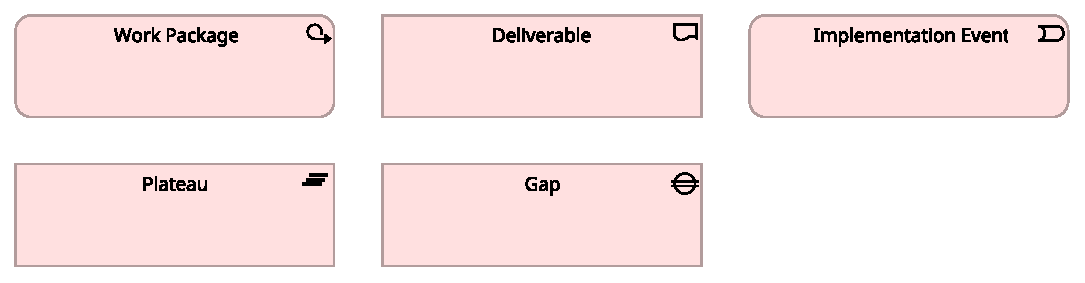
\includegraphics[width=\linewidth]{implementation-legend.pdf}
    \column{0.46\textwidth}
    \footnotesize
    \begin{itemize}\setlength{\itemsep}{3pt}
      \item \textbf{Work package} -- proyek/fase berawal-akhir jelas.
      \item \textbf{Deliverable} -- hasil kerja terdefinisi.
      \item \textbf{Implementation event} -- peristiwa (kickoff, go-live).
      \item \textbf{Plateau} -- keadaan arsitektur yang stabil.
      \item \textbf{Gap} -- selisih antar dua plateau.
    \end{itemize}
  \end{columns}
  \takeaway{Elemen migrasi berwarna merah muda; ikon pojok membedakan jenisnya.}
\end{frame}

\begin{frame}{Membedakan Elemen Migrasi}
  \vspace{4pt}
  {\footnotesize Contoh: rumah makan yang menambah kanal \textbf{pemesanan
  online}.}
  \begin{itemize}
    \item \textbf{Plateau:} \emph{keadaan}---``Baseline (pesan manual)'', ``Target
          (pemesanan online)''.
    \item \textbf{Gap:} \emph{selisih} antar keadaan---``Belum ada pemesanan
          online''.
    \item \textbf{Work package:} \emph{proyek}---``Proyek Pemesanan Online''.
    \item \textbf{Deliverable:} \emph{hasil}---``Aplikasi Pemesanan Online Live''.
    \item \textbf{Implementation event:} \emph{peristiwa}---``Peluncuran Layanan
          Online''.
  \end{itemize}
  \takeaway{Work package \emph{mewujudkan} deliverable; deliverable \emph{mewujudkan}
  plateau; plateau \emph{mencakup} kapabilitas; gap menandai selisih.}
\end{frame}

\begin{frame}{}
  \centering
  \vspace{1mm}
  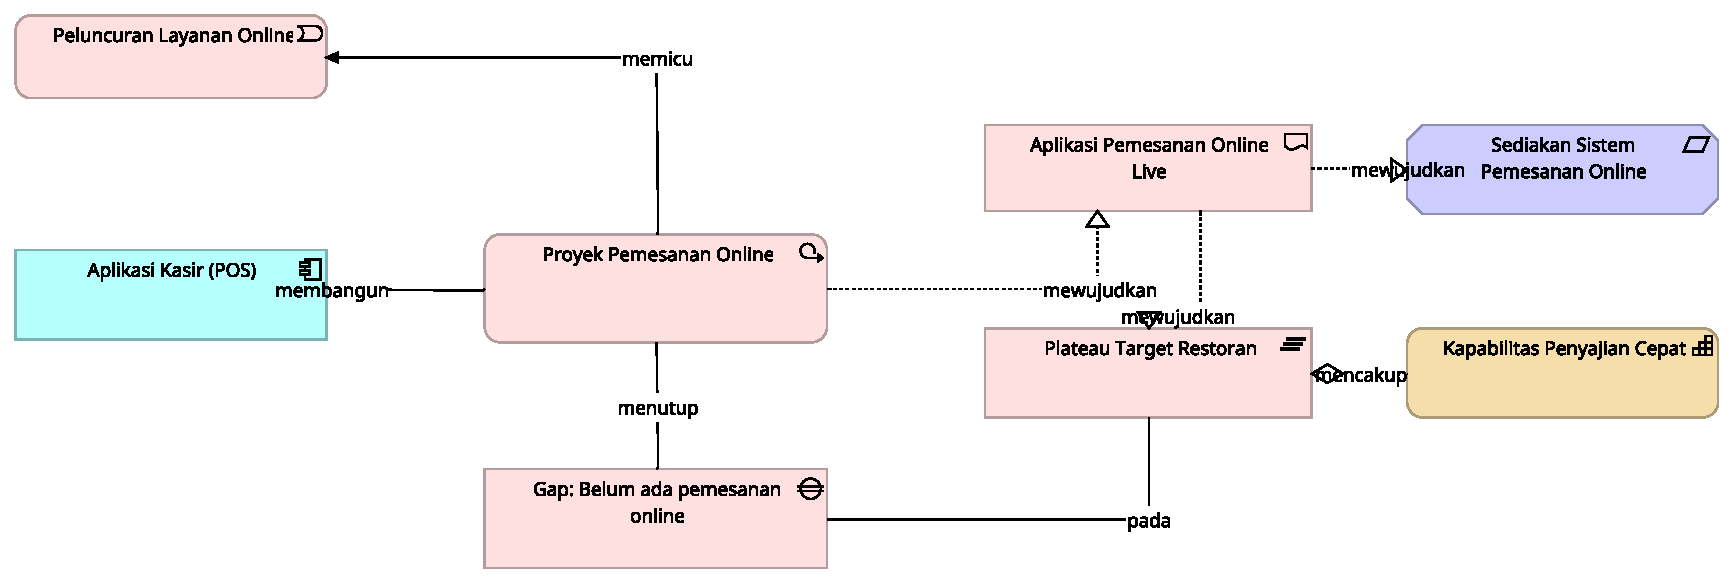
\includegraphics[width=\textwidth,height=.8\textheight,keepaspectratio]{implementation-contoh.pdf}\\
  {\scriptsize Contoh interaksi antar-elemen migrasi (kasus restoran): work package
  mewujudkan deliverable \& memicu peristiwa; deliverable mewujudkan plateau \&
  requirement; plateau mencakup kapabilitas; work package menutup gap.}
\end{frame}

% ============================================================
\section{Studi Kasus: Peta Jalan di Archi}
\sectionframe{Studi Kasus:\\ Peta Jalan Transformasi Bank Wanua}

\begin{frame}{}
  \centering
  \vspace{1mm}
  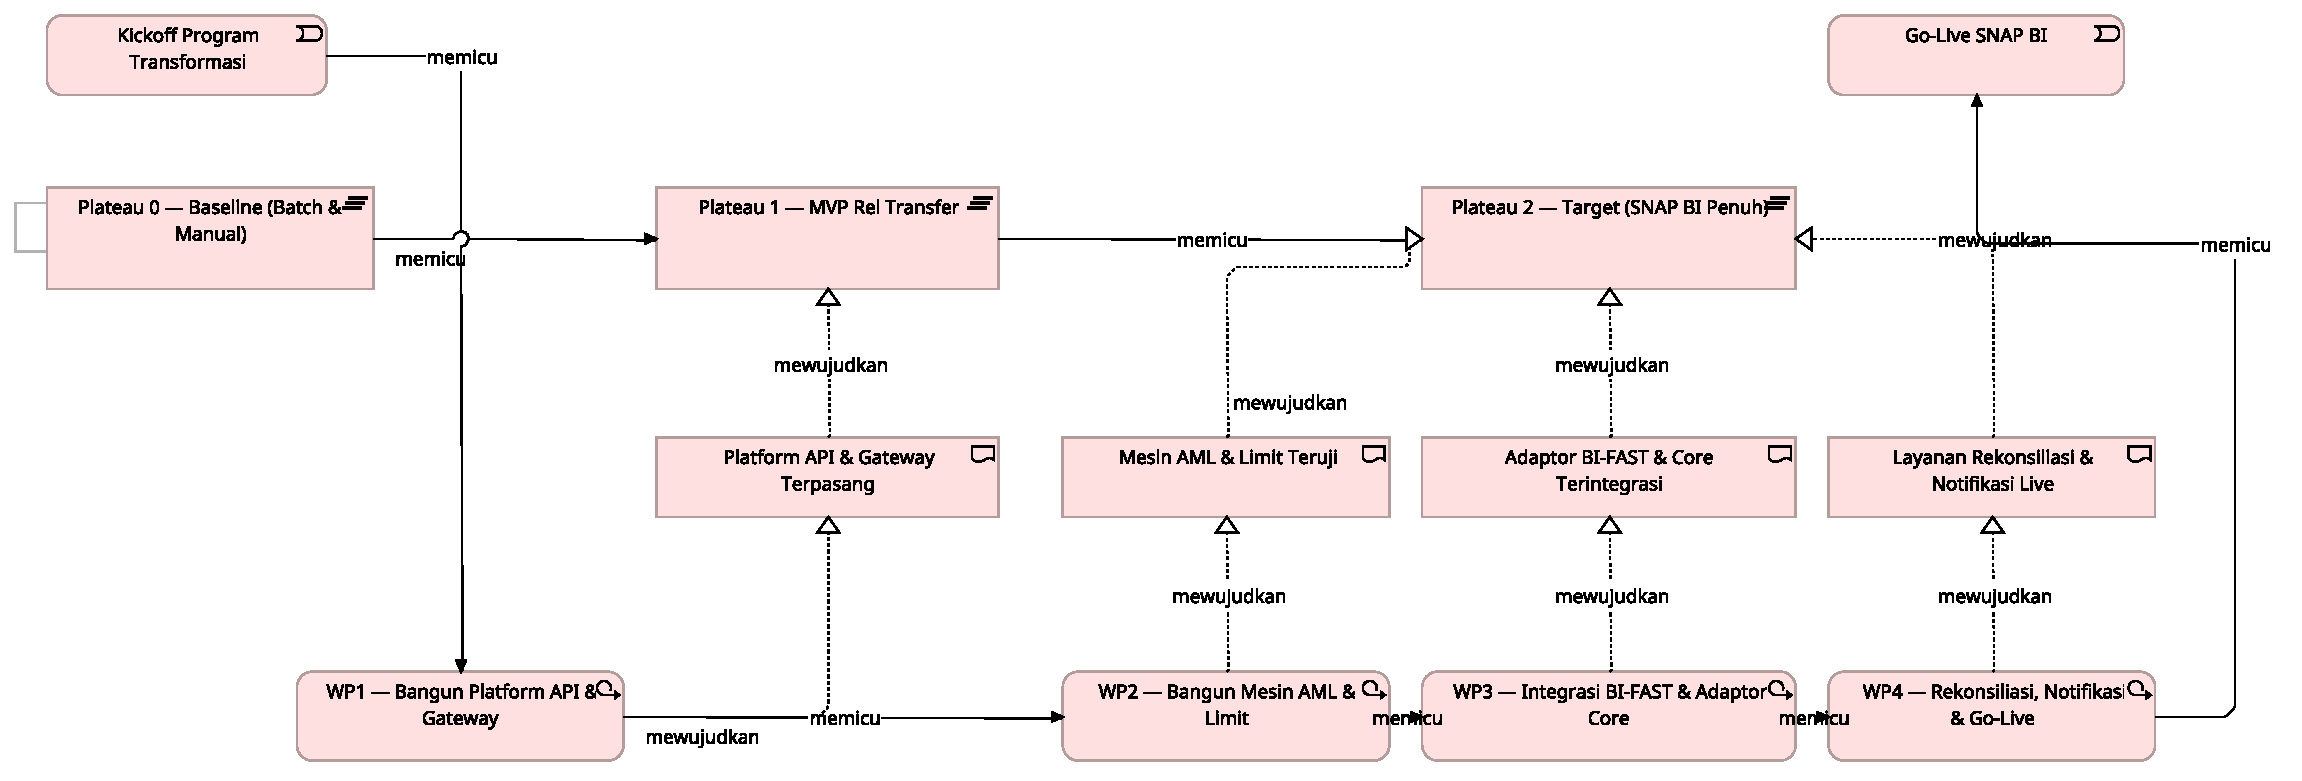
\includegraphics[width=\textwidth,height=.84\textheight,keepaspectratio]{implementation-roadmap.pdf}\\
  {\scriptsize Peta jalan: plateau Baseline $\rightarrow$ MVP $\rightarrow$ Target
  dipicu berurutan; tiap work package \emph{mewujudkan} deliverable yang
  \emph{mewujudkan} plateau; Kickoff dan Go-Live menandai tonggak.}
\end{frame}

\begin{frame}{}
  \centering
  \vspace{1mm}
  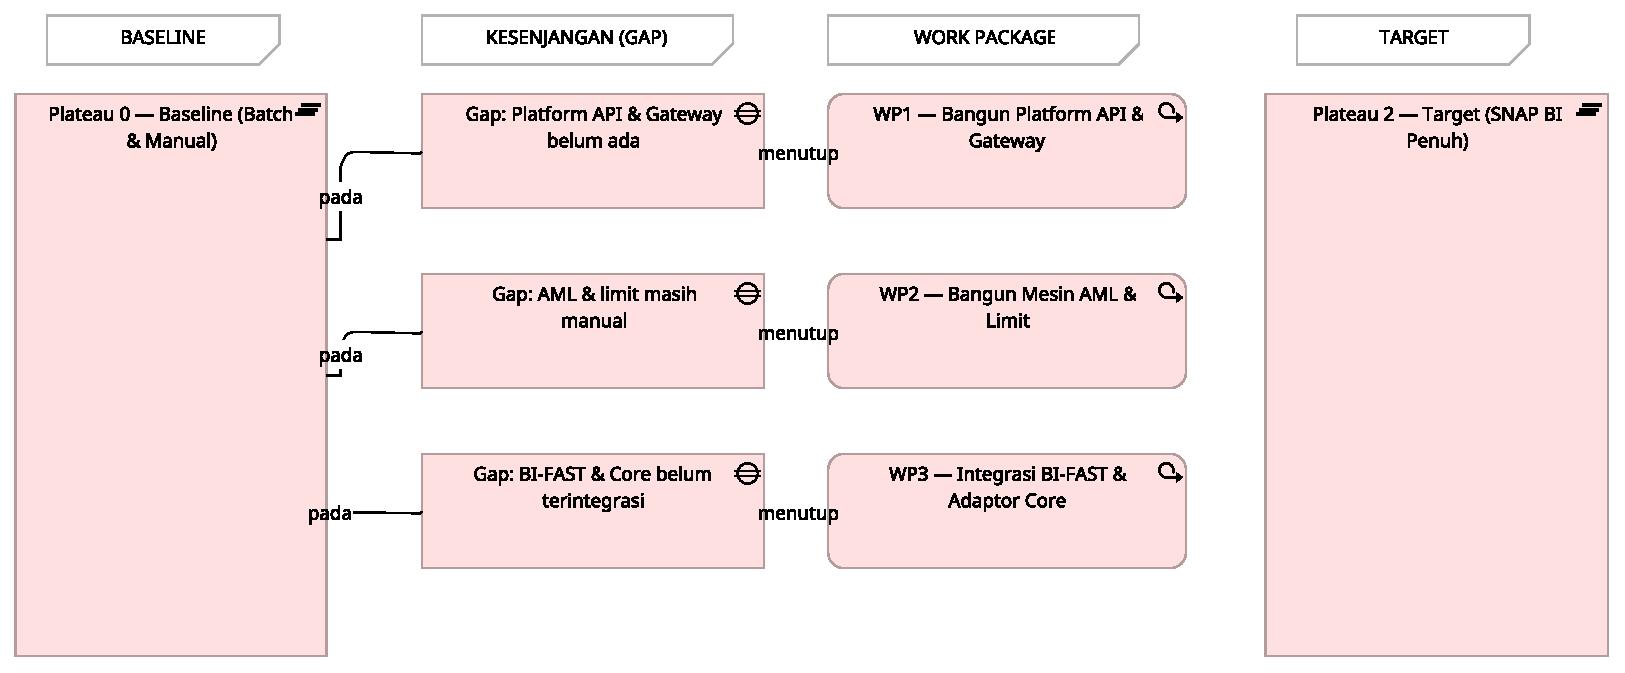
\includegraphics[width=\textwidth,height=.84\textheight,keepaspectratio]{implementation-gap.pdf}\\
  {\scriptsize Analisis kesenjangan: tiap \emph{gap} antara Baseline dan Target
  \emph{ditutup} oleh sebuah work package (TOGAF Fase E).}
\end{frame}

\begin{frame}{}
  \centering
  \vspace{1mm}
  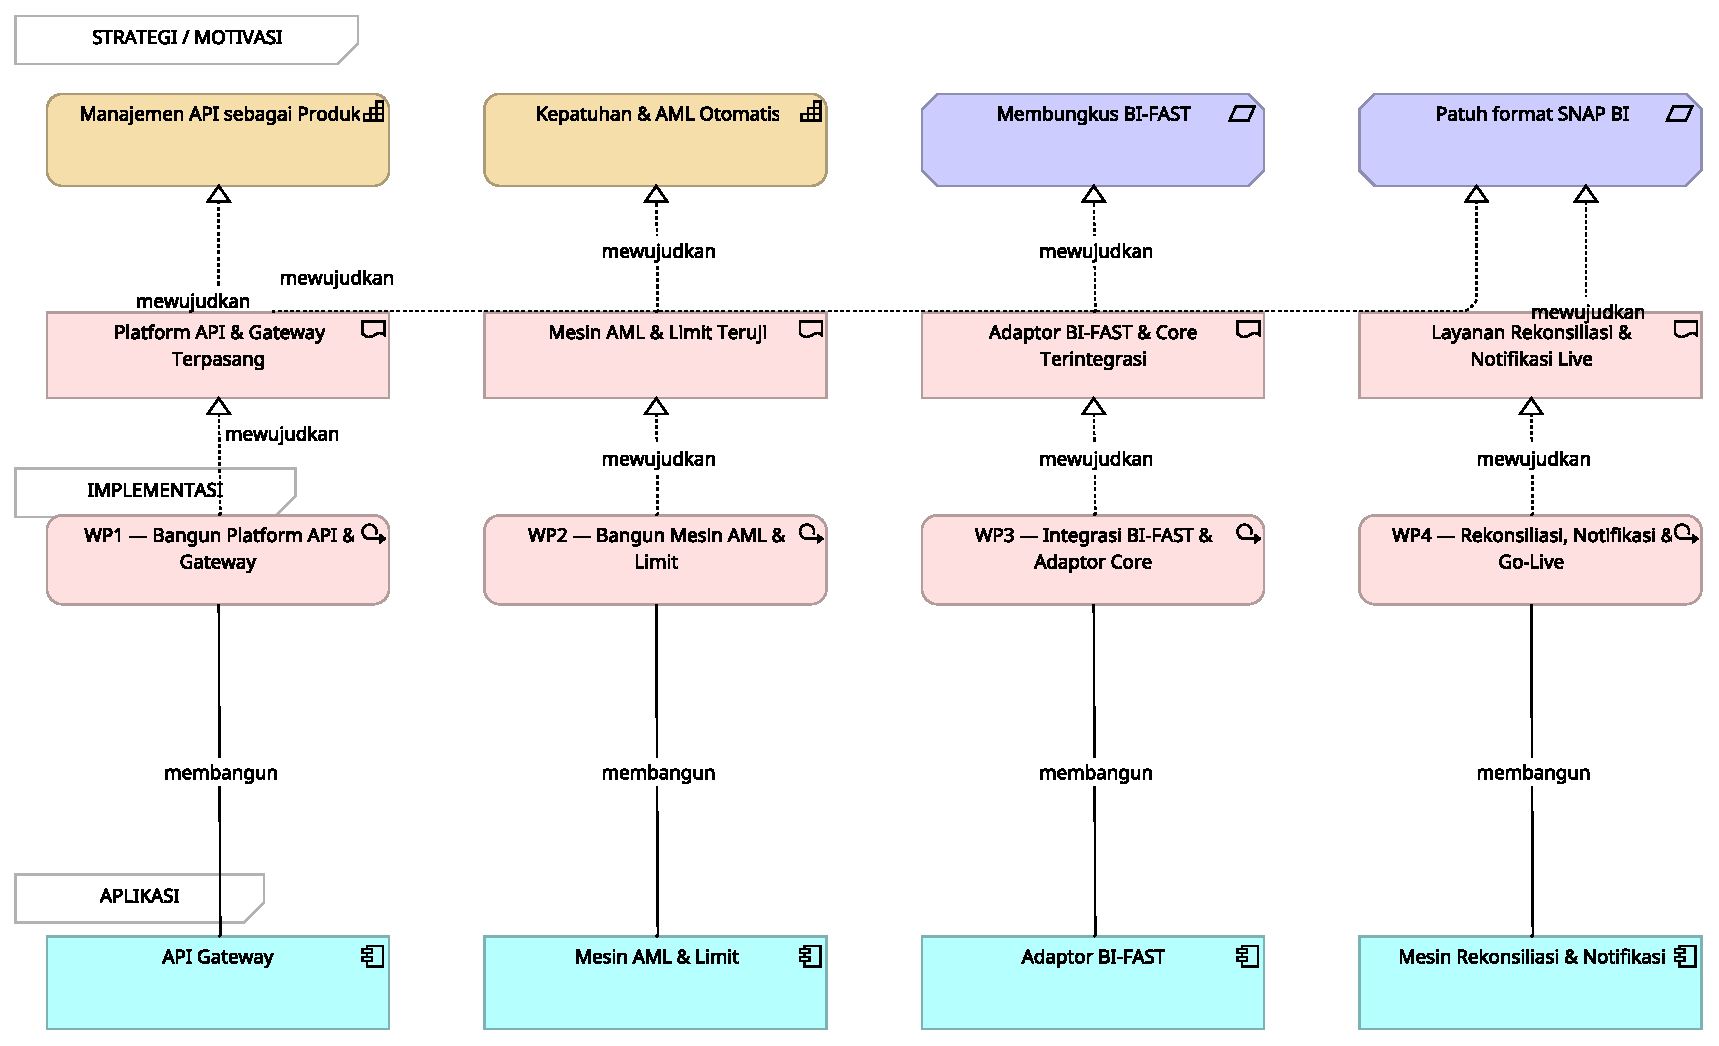
\includegraphics[width=\textwidth,height=.84\textheight,keepaspectratio]{implementation-stack.pdf}\\
  {\scriptsize Penyelarasan akhir: tiap work package \emph{membangun} komponen
  aplikasi, \emph{mewujudkan} deliverable; deliverable \emph{mewujudkan}
  kapabilitas/requirement strategi--motivasi.}
\end{frame}

\begin{frame}{Cara Membaca Peta Jalan}
  \vspace{4pt}
  \footnotesize
  \begin{itemize}\setlength{\itemsep}{2.5pt}
    \item \textbf{Triggering:} plateau \emph{memicu} plateau (Baseline
          $\rightarrow$ MVP $\rightarrow$ Target); work package berurutan.
    \item \textbf{Realisasi (WP):} work package \emph{mewujudkan} deliverable.
    \item \textbf{Realisasi (deliverable):} deliverable \emph{mewujudkan} plateau.
    \item \textbf{Agregasi:} plateau \emph{mencakup} kapabilitas/requirement yang
          aktif.
    \item \textbf{Asosiasi:} gap \emph{pada} baseline; work package \emph{menutup}
          gap \& \emph{membangun} komponen aplikasi.
  \end{itemize}
  \takeaway{Peristiwa (kickoff, go-live) menandai tonggak; tonggak kepatuhan
  (SNAP BI) menentukan urutan.}
\end{frame}

% ============================================================
\section{Latihan dan Penutup}
\sectionframe{Latihan dan Penutup}

\begin{frame}{Latihan Terapan Individual}
  \vspace{8pt}
  \begin{itemize}
    \item \textbf{Latihan 9.1} -- Baseline, target, dan gap.
    \item \textbf{Latihan 9.2} -- Work package \& deliverable (tautkan ke
          kapabilitas/requirement).
    \item \textbf{Latihan 9.3} -- Peta jalan berplateau (urutan \& tonggak).
    \item \textbf{Latihan 9.4} -- Paragraf rencana migrasi.
  \end{itemize}
  \takeaway{Semua latihan menjadi bahan langsung Rekomendasi \& Rencana makalah.}
\end{frame}

\begin{frame}{Penutup: Rantai Tujuh Lapisan}
  \vspace{6pt}
  \footnotesize
  \begin{itemize}\setlength{\itemsep}{2.0pt}
    \item \textbf{Motivasi} (mengapa) $\rightarrow$ \textbf{Strategi} $\rightarrow$
          \textbf{Bisnis} $\rightarrow$ \textbf{Data} $\rightarrow$
          \textbf{Aplikasi} $\rightarrow$ \textbf{Teknologi} (apa \& bagaimana)
          $\rightarrow$ \textbf{Implementasi \& Migrasi} (kapan \& dengan apa).
    \item Tiap lapisan \emph{menurun} dan \emph{mewujudkan} lapisan di atasnya;
          paket kerja membangunnya kembali menjadi kapabilitas.
    \item Satu model ArchiMate + TOGAF ADM yang tertelusuri dari ``mengapa''
          sampai ``kapan dan dengan apa''.
  \end{itemize}
  \takeaway{Menuntaskan tujuh lapisan pada satu studi kasus = sebuah arsitektur
  enterprise yang utuh, koheren, dan siap dipertahankan.}
\end{frame}

\begin{frame}{\hfill}
  \centering
  \Huge{\textbf{Terima kasih}}\\[8pt]
  \normalsize Pertanyaan \& diskusi
\end{frame}

\end{document}
